\documentclass[twoside]{book}

% Packages required by doxygen
\usepackage{fixltx2e}
\usepackage{calc}
\usepackage{doxygen}
\usepackage{graphicx}
\usepackage[utf8]{inputenc}
\usepackage{makeidx}
\usepackage{multicol}
\usepackage{multirow}
\PassOptionsToPackage{warn}{textcomp}
\usepackage{textcomp}
\usepackage[nointegrals]{wasysym}
\usepackage[table]{xcolor}

% Font selection
\usepackage[T1]{fontenc}
\usepackage{mathptmx}
\usepackage[scaled=.90]{helvet}
\usepackage{courier}
\usepackage{amssymb}
\usepackage{sectsty}
\renewcommand{\familydefault}{\sfdefault}
\allsectionsfont{%
  \fontseries{bc}\selectfont%
  \color{darkgray}%
}
\renewcommand{\DoxyLabelFont}{%
  \fontseries{bc}\selectfont%
  \color{darkgray}%
}
\newcommand{\+}{\discretionary{\mbox{\scriptsize$\hookleftarrow$}}{}{}}

% Page & text layout
\usepackage{geometry}
\geometry{%
  a4paper,%
  top=2.5cm,%
  bottom=2.5cm,%
  left=2.5cm,%
  right=2.5cm%
}
\tolerance=750
\hfuzz=15pt
\hbadness=750
\setlength{\emergencystretch}{15pt}
\setlength{\parindent}{0cm}
\setlength{\parskip}{0.2cm}
\makeatletter
\renewcommand{\paragraph}{%
  \@startsection{paragraph}{4}{0ex}{-1.0ex}{1.0ex}{%
    \normalfont\normalsize\bfseries\SS@parafont%
  }%
}
\renewcommand{\subparagraph}{%
  \@startsection{subparagraph}{5}{0ex}{-1.0ex}{1.0ex}{%
    \normalfont\normalsize\bfseries\SS@subparafont%
  }%
}
\makeatother

% Headers & footers
\usepackage{fancyhdr}
\pagestyle{fancyplain}
\fancyhead[LE]{\fancyplain{}{\bfseries\thepage}}
\fancyhead[CE]{\fancyplain{}{}}
\fancyhead[RE]{\fancyplain{}{\bfseries\leftmark}}
\fancyhead[LO]{\fancyplain{}{\bfseries\rightmark}}
\fancyhead[CO]{\fancyplain{}{}}
\fancyhead[RO]{\fancyplain{}{\bfseries\thepage}}
\fancyfoot[LE]{\fancyplain{}{}}
\fancyfoot[CE]{\fancyplain{}{}}
\fancyfoot[RE]{\fancyplain{}{\bfseries\scriptsize Generated on Fri Oct 21 2016 09\+:18\+:26 for Proyecto1 by Doxygen }}
\fancyfoot[LO]{\fancyplain{}{\bfseries\scriptsize Generated on Fri Oct 21 2016 09\+:18\+:26 for Proyecto1 by Doxygen }}
\fancyfoot[CO]{\fancyplain{}{}}
\fancyfoot[RO]{\fancyplain{}{}}
\renewcommand{\footrulewidth}{0.4pt}
\renewcommand{\chaptermark}[1]{%
  \markboth{#1}{}%
}
\renewcommand{\sectionmark}[1]{%
  \markright{\thesection\ #1}%
}

% Indices & bibliography
\usepackage{natbib}
\usepackage[titles]{tocloft}
\setcounter{tocdepth}{3}
\setcounter{secnumdepth}{5}
\makeindex

% Hyperlinks (required, but should be loaded last)
\usepackage{ifpdf}
\ifpdf
  \usepackage[pdftex,pagebackref=true]{hyperref}
\else
  \usepackage[ps2pdf,pagebackref=true]{hyperref}
\fi
\hypersetup{%
  colorlinks=true,%
  linkcolor=blue,%
  citecolor=blue,%
  unicode%
}

% Custom commands
\newcommand{\clearemptydoublepage}{%
  \newpage{\pagestyle{empty}\cleardoublepage}%
}


%===== C O N T E N T S =====

\begin{document}

% Titlepage & ToC
\hypersetup{pageanchor=false,
             bookmarks=true,
             bookmarksnumbered=true,
             pdfencoding=unicode
            }
\pagenumbering{roman}
\begin{titlepage}
\vspace*{7cm}
\begin{center}%
{\Large Proyecto1 }\\
\vspace*{1cm}
{\large Generated by Doxygen 1.8.8}\\
\vspace*{0.5cm}
{\small Fri Oct 21 2016 09:18:26}\\
\end{center}
\end{titlepage}
\clearemptydoublepage
\tableofcontents
\clearemptydoublepage
\pagenumbering{arabic}
\hypersetup{pageanchor=true}

%--- Begin generated contents ---
\chapter{Class Index}
\section{Class List}
Here are the classes, structs, unions and interfaces with brief descriptions\+:\begin{DoxyCompactList}
\item\contentsline{section}{\hyperlink{class_juego_de_la_vida}{Juego\+De\+La\+Vida} }{\pageref{class_juego_de_la_vida}}{}
\end{DoxyCompactList}

\chapter{Class Documentation}
\hypertarget{class_juego_de_la_vida}{\section{Juego\+De\+La\+Vida Class Reference}
\label{class_juego_de_la_vida}\index{Juego\+De\+La\+Vida@{Juego\+De\+La\+Vida}}
}


Collaboration diagram for Juego\+De\+La\+Vida\+:
\nopagebreak
\begin{figure}[H]
\begin{center}
\leavevmode
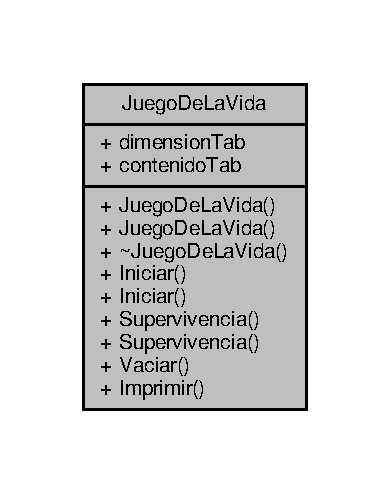
\includegraphics[width=187pt]{class_juego_de_la_vida__coll__graph}
\end{center}
\end{figure}
\subsection*{Public Member Functions}
\begin{DoxyCompactItemize}
\item 
\hypertarget{class_juego_de_la_vida_abdf075de6a4d6846add00de43e7d76ef}{\hyperlink{class_juego_de_la_vida_abdf075de6a4d6846add00de43e7d76ef}{Juego\+De\+La\+Vida} ()}\label{class_juego_de_la_vida_abdf075de6a4d6846add00de43e7d76ef}

\begin{DoxyCompactList}\small\item\em Constructor vacío de \hyperlink{class_juego_de_la_vida}{Juego\+De\+La\+Vida}. \end{DoxyCompactList}\item 
\hypertarget{class_juego_de_la_vida_a01b02de60c1f09ff38bcaf6c599eddaa}{\hyperlink{class_juego_de_la_vida_a01b02de60c1f09ff38bcaf6c599eddaa}{Juego\+De\+La\+Vida} (int \hyperlink{class_juego_de_la_vida_a1ed9d7c192843b0414ed8d0d221427bc}{dimension\+Tab}, int $\ast$$\ast$contenido\+Tab)}\label{class_juego_de_la_vida_a01b02de60c1f09ff38bcaf6c599eddaa}

\begin{DoxyCompactList}\small\item\em Constructor de \hyperlink{class_juego_de_la_vida}{Juego\+De\+La\+Vida}. \end{DoxyCompactList}\item 
virtual \hyperlink{class_juego_de_la_vida_af78ed62608dd32d4f7043ad45b599dc2}{$\sim$\+Juego\+De\+La\+Vida} ()
\begin{DoxyCompactList}\small\item\em Desctructor de \hyperlink{class_juego_de_la_vida}{Juego\+De\+La\+Vida}. \end{DoxyCompactList}\item 
void \hyperlink{class_juego_de_la_vida_a84dbec00b828b6102bb445f5103a1bed}{Iniciar} (\hyperlink{class_juego_de_la_vida}{Juego\+De\+La\+Vida} \&)
\begin{DoxyCompactList}\small\item\em Funciones de \hyperlink{class_juego_de_la_vida}{Juego\+De\+La\+Vida}. \end{DoxyCompactList}\item 
void \hyperlink{class_juego_de_la_vida_aeb29d8845eadc2de5cb12112c1fa1d59}{Iniciar} (\hyperlink{class_juego_de_la_vida}{Juego\+De\+La\+Vida} \&, int Num\+Gen)
\item 
void \hyperlink{class_juego_de_la_vida_adbfe5f4086c938071f99082ea5ee6039}{Supervivencia} (\hyperlink{class_juego_de_la_vida}{Juego\+De\+La\+Vida} \&, int $\ast$$\ast$cont\+Temporal)
\item 
void \hyperlink{class_juego_de_la_vida_a78b5f60ad9b7830ff3cba3f60dcf31b6}{Supervivencia} (\hyperlink{class_juego_de_la_vida}{Juego\+De\+La\+Vida} \&, int $\ast$$\ast$cont\+Temporal, int Num\+Gen)
\item 
\hypertarget{class_juego_de_la_vida_a4a55e27a01a746aa7a2da352dd2c82ca}{void {\bfseries Vaciar} (\hyperlink{class_juego_de_la_vida}{Juego\+De\+La\+Vida} \&)}\label{class_juego_de_la_vida_a4a55e27a01a746aa7a2da352dd2c82ca}

\item 
\hypertarget{class_juego_de_la_vida_a138082a61e1414ff99cad59c64907fa9}{void {\bfseries Imprimir} (const \hyperlink{class_juego_de_la_vida}{Juego\+De\+La\+Vida} \&)}\label{class_juego_de_la_vida_a138082a61e1414ff99cad59c64907fa9}

\end{DoxyCompactItemize}
\subsection*{Public Attributes}
\begin{DoxyCompactItemize}
\item 
\hypertarget{class_juego_de_la_vida_a1ed9d7c192843b0414ed8d0d221427bc}{int \hyperlink{class_juego_de_la_vida_a1ed9d7c192843b0414ed8d0d221427bc}{dimension\+Tab}}\label{class_juego_de_la_vida_a1ed9d7c192843b0414ed8d0d221427bc}

\begin{DoxyCompactList}\small\item\em Atributos de \hyperlink{class_juego_de_la_vida}{Juego\+De\+La\+Vida}. \end{DoxyCompactList}\item 
\hypertarget{class_juego_de_la_vida_ac5dc03a87e1bb4e2c5ba72b445aed701}{int $\ast$$\ast$ {\bfseries contenido\+Tab}}\label{class_juego_de_la_vida_ac5dc03a87e1bb4e2c5ba72b445aed701}

\end{DoxyCompactItemize}


\subsection{Constructor \& Destructor Documentation}
\hypertarget{class_juego_de_la_vida_af78ed62608dd32d4f7043ad45b599dc2}{\index{Juego\+De\+La\+Vida@{Juego\+De\+La\+Vida}!````~Juego\+De\+La\+Vida@{$\sim$\+Juego\+De\+La\+Vida}}
\index{````~Juego\+De\+La\+Vida@{$\sim$\+Juego\+De\+La\+Vida}!Juego\+De\+La\+Vida@{Juego\+De\+La\+Vida}}
\subsubsection[{$\sim$\+Juego\+De\+La\+Vida}]{\setlength{\rightskip}{0pt plus 5cm}Juego\+De\+La\+Vida\+::$\sim$\+Juego\+De\+La\+Vida (
\begin{DoxyParamCaption}
{}
\end{DoxyParamCaption}
)\hspace{0.3cm}{\ttfamily [virtual]}}}\label{class_juego_de_la_vida_af78ed62608dd32d4f7043ad45b599dc2}


Desctructor de \hyperlink{class_juego_de_la_vida}{Juego\+De\+La\+Vida}. 

Destructor de \hyperlink{class_juego_de_la_vida}{Juego\+De\+La\+Vida}. 

\subsection{Member Function Documentation}
\hypertarget{class_juego_de_la_vida_a84dbec00b828b6102bb445f5103a1bed}{\index{Juego\+De\+La\+Vida@{Juego\+De\+La\+Vida}!Iniciar@{Iniciar}}
\index{Iniciar@{Iniciar}!Juego\+De\+La\+Vida@{Juego\+De\+La\+Vida}}
\subsubsection[{Iniciar}]{\setlength{\rightskip}{0pt plus 5cm}void Juego\+De\+La\+Vida\+::\+Iniciar (
\begin{DoxyParamCaption}
\item[{{\bf Juego\+De\+La\+Vida} \&}]{}
\end{DoxyParamCaption}
)}}\label{class_juego_de_la_vida_a84dbec00b828b6102bb445f5103a1bed}


Funciones de \hyperlink{class_juego_de_la_vida}{Juego\+De\+La\+Vida}. 

Construcción arreglo 2d para el Tablero temporal

Inicialización valores Tablero temporal \hypertarget{class_juego_de_la_vida_aeb29d8845eadc2de5cb12112c1fa1d59}{\index{Juego\+De\+La\+Vida@{Juego\+De\+La\+Vida}!Iniciar@{Iniciar}}
\index{Iniciar@{Iniciar}!Juego\+De\+La\+Vida@{Juego\+De\+La\+Vida}}
\subsubsection[{Iniciar}]{\setlength{\rightskip}{0pt plus 5cm}void Juego\+De\+La\+Vida\+::\+Iniciar (
\begin{DoxyParamCaption}
\item[{{\bf Juego\+De\+La\+Vida} \&}]{, }
\item[{int}]{Num\+Gen}
\end{DoxyParamCaption}
)}}\label{class_juego_de_la_vida_aeb29d8845eadc2de5cb12112c1fa1d59}
Construcción arreglo 2d para el Tablero temporal

Inicialización valores Tablero temporal \hypertarget{class_juego_de_la_vida_adbfe5f4086c938071f99082ea5ee6039}{\index{Juego\+De\+La\+Vida@{Juego\+De\+La\+Vida}!Supervivencia@{Supervivencia}}
\index{Supervivencia@{Supervivencia}!Juego\+De\+La\+Vida@{Juego\+De\+La\+Vida}}
\subsubsection[{Supervivencia}]{\setlength{\rightskip}{0pt plus 5cm}void Juego\+De\+La\+Vida\+::\+Supervivencia (
\begin{DoxyParamCaption}
\item[{{\bf Juego\+De\+La\+Vida} \&}]{, }
\item[{int $\ast$$\ast$}]{cont\+Temporal}
\end{DoxyParamCaption}
)}}\label{class_juego_de_la_vida_adbfe5f4086c938071f99082ea5ee6039}
Renacimiento celulas

Supervivencia celulas

Igualación contenido a contenido temporal \hypertarget{class_juego_de_la_vida_a78b5f60ad9b7830ff3cba3f60dcf31b6}{\index{Juego\+De\+La\+Vida@{Juego\+De\+La\+Vida}!Supervivencia@{Supervivencia}}
\index{Supervivencia@{Supervivencia}!Juego\+De\+La\+Vida@{Juego\+De\+La\+Vida}}
\subsubsection[{Supervivencia}]{\setlength{\rightskip}{0pt plus 5cm}void Juego\+De\+La\+Vida\+::\+Supervivencia (
\begin{DoxyParamCaption}
\item[{{\bf Juego\+De\+La\+Vida} \&}]{, }
\item[{int $\ast$$\ast$}]{cont\+Temporal, }
\item[{int}]{Num\+Gen}
\end{DoxyParamCaption}
)}}\label{class_juego_de_la_vida_a78b5f60ad9b7830ff3cba3f60dcf31b6}
Renacimiento celulas

Supervivencia celulas

Igualación contenido a contenido temporal 

The documentation for this class was generated from the following files\+:\begin{DoxyCompactItemize}
\item 
Juego\+De\+La\+Vida.\+h\item 
Juego\+De\+La\+Vida.\+cpp\end{DoxyCompactItemize}

%--- End generated contents ---

% Index
\newpage
\phantomsection
\addcontentsline{toc}{chapter}{Index}
\printindex

\end{document}
